\chapter{Host Compiled Simulation}

\gls{hcs} is based on the approach of Source Code Instrumentation (SCI). Instrumentation is the technique to modify the source code of an application, in order to extract debug or trace information at run-time. In \gls{hcs}, the source code is instrumented to estimate the time spent in executing the application on a particular target processor. 

When an application is run on a processor, most of the time is spent in following phases.
\begin{itemize} \itemsep -6pt
\item Execution of instructions.
\item Fetching Data from memory.
\end{itemize}

The technique is based on the assumption, that number of cycles spent in each phase of the execution can be accurately predicted using instrumentation. The trace generated from the run-time can be used for estimating the power consumption.

The information generated is useful for architects to analyse the impact of design decisions on performance and power consumption of the system. In comparison to popular techniques like Cycle Accurate Simulation (CAS), \gls{hcs} is easier to develop and fast to execute. This greatly optimizes the design space exploration effort.

In this chapter, the concept of \gls{hcs} is illustrated using a simplified example. The steps involved in performing \gls{hcs} are outlined. Further, an overview of each step is provided. Detailed implementation of each step has been discussed in the next chapter.

\section{Simple Example}
\label{sec:SimpleExample}
Consider the source code in Listing \ref{lst:sumCCode}. The function \emph{sum} calculates the sum of elements in an array and returns the result. The source code is cross-compiled for a target processor\footnote{Target processor is the processor that is being simulated.}. Listing \ref{lst:sumObjCode} shows the object dump of the binary code. 

To estimate the time spent in executing this code on the target processor, the code is instrumented. The instrumented code is shown in Listing \ref{lst:sumInstCode}, where the annotations are highlighted. The instrumented code is then compiled for and run on the host machine\footnote{Host Machine is the computer used by the developer, where the simulation will be run.}. This process is called Host Compiled Simulation. Let us look at each annotation in the code.

\vspace*{10pt}
\begin{minipage}{0.5\textwidth}
\begin{lstlisting}[caption={Simple C Code},label={lst:sumCCode}]
int sum(int array[20])
{
	int i;
	int sum = 0;
	
	for (i=0; i<20; i++)
		sum += array[i];
	
	return sum;
}
\end{lstlisting}
\end{minipage}%
\begin{minipage}{0.5\textwidth}
\begin{lstlisting}[caption={Objdump Code},label={lst:sumObjCode}]
00008068 <sum>:
8068:     mov     r3, #0
806c:     mov     r2, r3
8070:     ldr     r1, [r0, r3]
8074:     add     r2, r2, r1
8078:     add     r3, r3, #4
807c:     cmp     r3, #80 ; 0x50
8080:     bne     8070 <sum+0x8>
8084:     mov     r0, r2
8088:     bx      lr
\end{lstlisting}
\end{minipage}
\vspace*{5pt}
\begin{lstlisting}[caption={Instrumented Code},label={lst:sumInstCode}]
`unsigned int execCycles;`
`unsigned int memAccessCycles;`

int sum(int array[20])
{
	int i;
	int sum = 0;
	`execCycles += 2;`
	`memAccessCycles += simICache(0x8068, 8);`
	
	for (i=0; i<20; i++)
	{
		sum += array[i];
		`memAccessCycles += simDCache(&array + i, READ);`
		`execCycles += 5;`
		`memAccessCycles += simICache(0x8070, 40);`
	}
	
	`execCycles += 2;`
	`memAccessCycles += simICache(0x8084, 8);`
	return sum;
}
\end{lstlisting}

In the instrumented code, two global variables \emph{execCycles} and \emph{memAccessCycles} have been declared on lines 1 and 2 respectively. \emph{execCycles} will store the number of cycles spent in actual execution of instructions, when the processor is in active state. \emph{memAccessCycles} will store the number of cycles spent in performing read/write operations to the memory.

For accurate instrumentation, mapping  at basic block\footnote{Basic Block is a portion of the binary code with only one entry point and one exit point. A basic block can not contain any branch instructions.} granularity is needed between source code and binary code. From the binary code, three basic blocks can be identified. These blocks are mapped to corresponding blocks in the source code by static analysis. The mapping is shown in the Table \ref{tbl:ExMapping}.

\vspace*{15pt}
\begin{table}[h]
\begin{center}
\begin{tabularx}{320pt}{>{\centering\arraybackslash}X>{\centering\arraybackslash}X>{\centering\arraybackslash}X>{\centering\arraybackslash}X}
\toprule
	\multicolumn{2}{c}{Basic Block in Binary} & \multicolumn{2}{c}{Matching block in Source}\\ 
	\midrule
	BlockID & Lines & BlockID & Lines \\
    \hline
	1 & 1-2 & 1 & 3-4 \\
	2 & 4-8 & 2 & 7 \\
	3 & 9-10 & 3 & 9 \\	
\bottomrule
\end{tabularx}
\caption{Mapping of Basic Blocks}
\label{tbl:ExMapping}
\end{center}
\end{table}

Time spent in executing the instructions needs to be accounted. For simplicity, let us assume that the target processor executes each instruction in one cycle, and there is no latency in accessing memory. The number of cycles spent in execution of each basic block can be estimated by static analysis. Each basic block is annotated as seen on lines 8, 15 and 19 to accumulate the total cycles spent in the global variable \emph{execCycles}.

To accurately account for the cycles spent in accessing memory, the cache-hierarchy on the target processor needs to be simulated at run-time. Each load/store operation in the binary code is identified. Annotation is added to the source code to simulate the load/store operation. The cache simulator offers the API \emph{simDCache} to simulate data access. It takes as parameter the \emph{address} of the data and a \emph{flag} to tell whether it is a read or write access. The cycles spent in performing the memory access is returned.

A load operation is identified on line 4 in the object code. This corresponds to loading of elements of \emph{array}. The operation is simulated by the annotation on line 14 in the instrumented code. The return value from the cache simulator is accumulated in the global variable \emph{memAccessCycles}.

The cycles spent in fetching instructions from the memory must also be accounted. This is done at the basic block granularity. The cache simulator offers API \emph{simICache} which takes as parameters \emph{address} of the first instructions in the basic block, and \emph{size} of the basic block in bytes. The cache simulator returns the number of cycles spent in fetching the instructions. Annotation for simulating instruction cache access is seen on lines 9, 16 and 20.

This instrumented code is compiled for and run on the Host Machine. The values of \emph{execCycles} and \emph{memAccessCycles} are delivered at the end. 

The following sections will build upon this basic concept. Modern processors are more complicated than the target processor used for this illustration. The features of the modern processors will need to be simulated in sufficient detail to extract accurate estimates of performance.

\section{The Flow}

Figure \ref{fig:hcsFlowChart} shows a flow-chart depicting the stages involved in performing automatic instrumentation. Each stage is explained in further sections.

\begin{figure}[h!]
\center
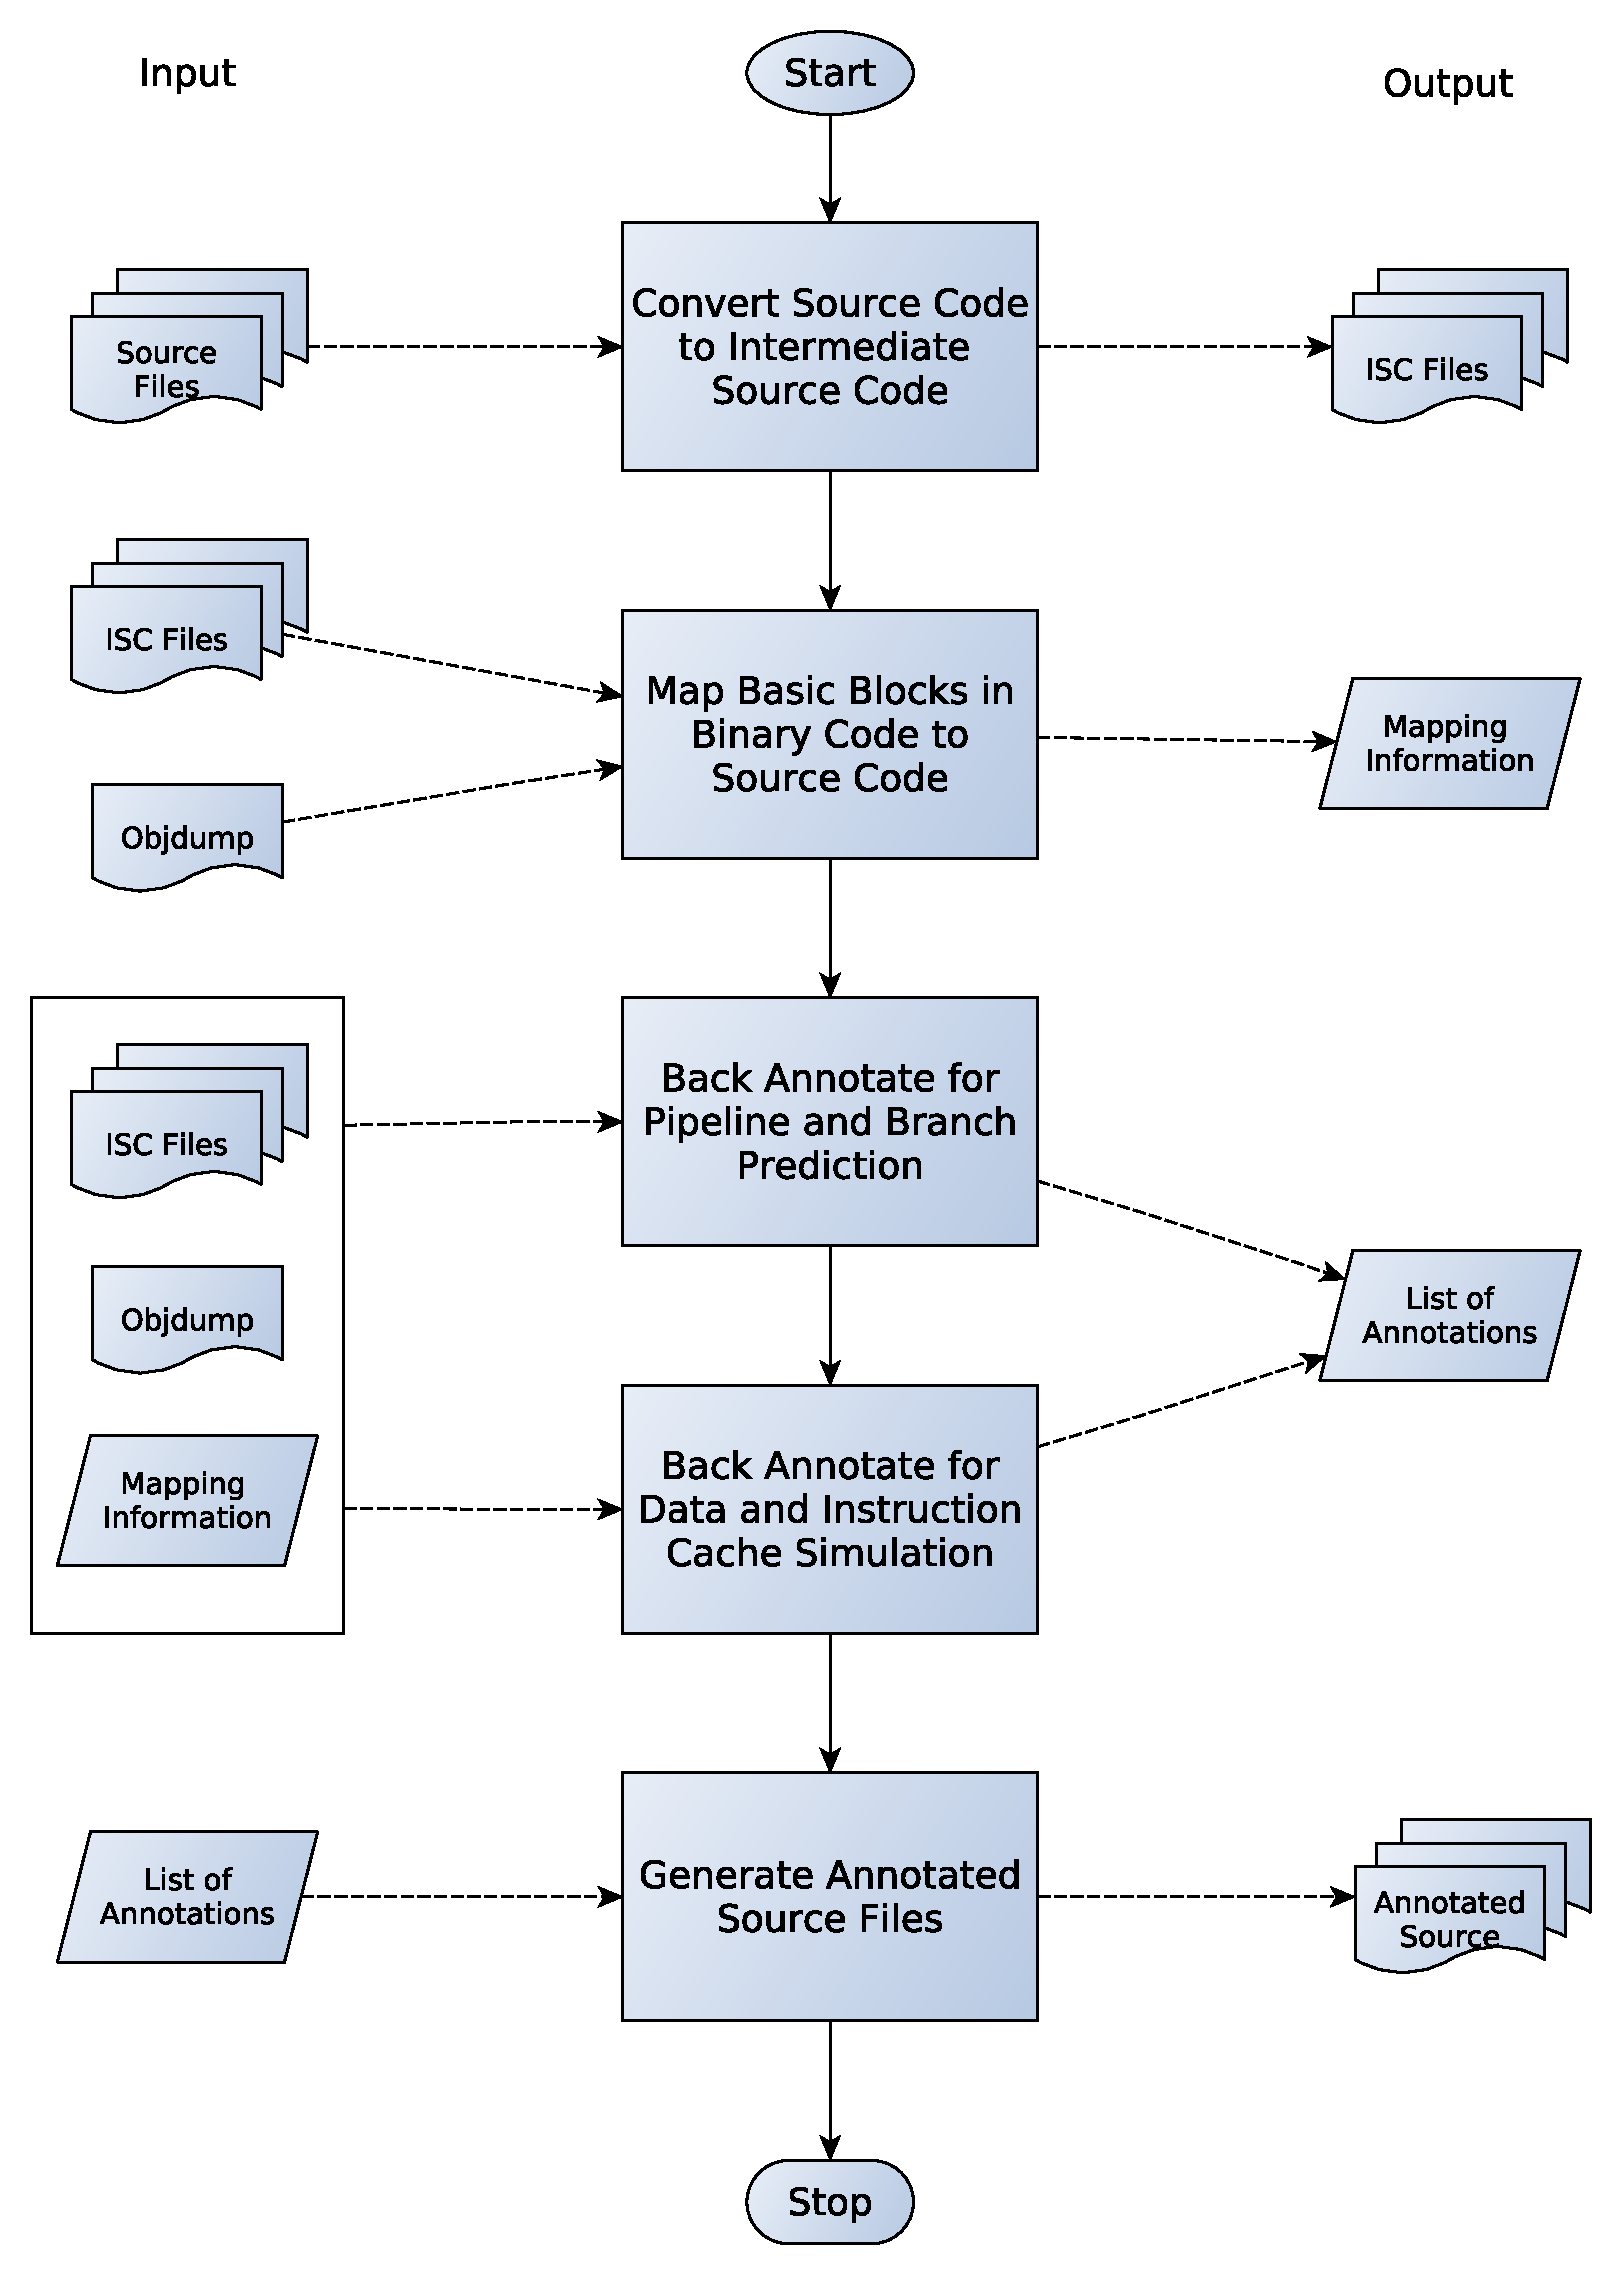
\includegraphics[width=.9\textwidth]{figures/HCS_FlowChart.pdf}
\caption{Flow Chart}
\label{fig:hcsFlowChart}
\end{figure}

%In this section, a brief overview of the project architecture is provided. Each part of the project is independent, and has been treated as a separate problem. The flow chart in figure [TODO] shows each step of the project. The approach to solve these techniques is presented in the subsequent sections in this chapter. Details of the implementation have been presented in the next chapter.

%From the example, it is clear that for correctly instrumenting the code accurate mapping is required between the source code and the binary code. However, this mapping is usually destroyed during the optimization phases of the compiler. The first problem that is solved in this project is to generate accurate mapping information at the Basic Block granularity. 
%
%In the next step, GDB is used to derive information about each variable that is used in the application. During compiler optimization, most of the variables defined by the user are optimized out, hence this information can only be extracted from the debug information with the binary code. Names, addresses and sizes of Global and Local Variables are extracted.
%
%For simulating data cache, each load and store instruction is accurately matched to an instruction in the source code. The variable being accessed is identified, and the annotation to simulate the memory access is added to the code. For simulating the instruction cache, annotation is added for each basic block in the binary code to the corresponding basic block in the source code.
%
%To estimate the amount of cycles spent in execution of a basic block in the processor pipeline, each instruction in a basic block is sequentially parsed to identify interlocking. Interlocking occurs when there is a Control or Data Dependency between instructions, which results in pipeline stall for a few cycles. The cycles used by each basic block are annotated back to the code. Further, a mechanism to emulate Branch Prediction Unit has been implemented. 

\section{Source Code to Intermediate Source Code}
From the example, it is clear that accurate mapping between source code and binary code is very important for instrumentation. Unfortunately, this mapping is destroyed during the optimization phases of the compiler. Extracting accurate mapping information is a challenging problem. In this project, an approach recommended in [TODO] has been used to reduce the complexity of this problem.

The compiler performs these optimizations in two stages. The front-end of the compiler, translates the source code from a high-level language like C, to an Intermediate Representation (IR) called GIMPLE. The processor independent optimization strategies are applied to the IR code. In the back-end of the compiler, the optimized IR code is translated into Machine Language for the target processor. The processor dependent optimization strategies are applied in this phase.

The optimized IR Code has a control flow similar to that of the Binary Code, since front-end optimization strategies have already been applied. It should be comparatively easier to perform mapping between the IR Code and the Binary Code. However, instrumentation of IR Code is difficult as it is in the GIMPLE format. 

In this project, the source code of the benchmark application is cross-compiled, and the optimized IR Code is translated back into a high-level language, C. The generated code is called \gls{isc}. The code to convert GIMPLE code to C code has been reused from \cite{RBA2013}.

\begin{figure}[h]
\centering
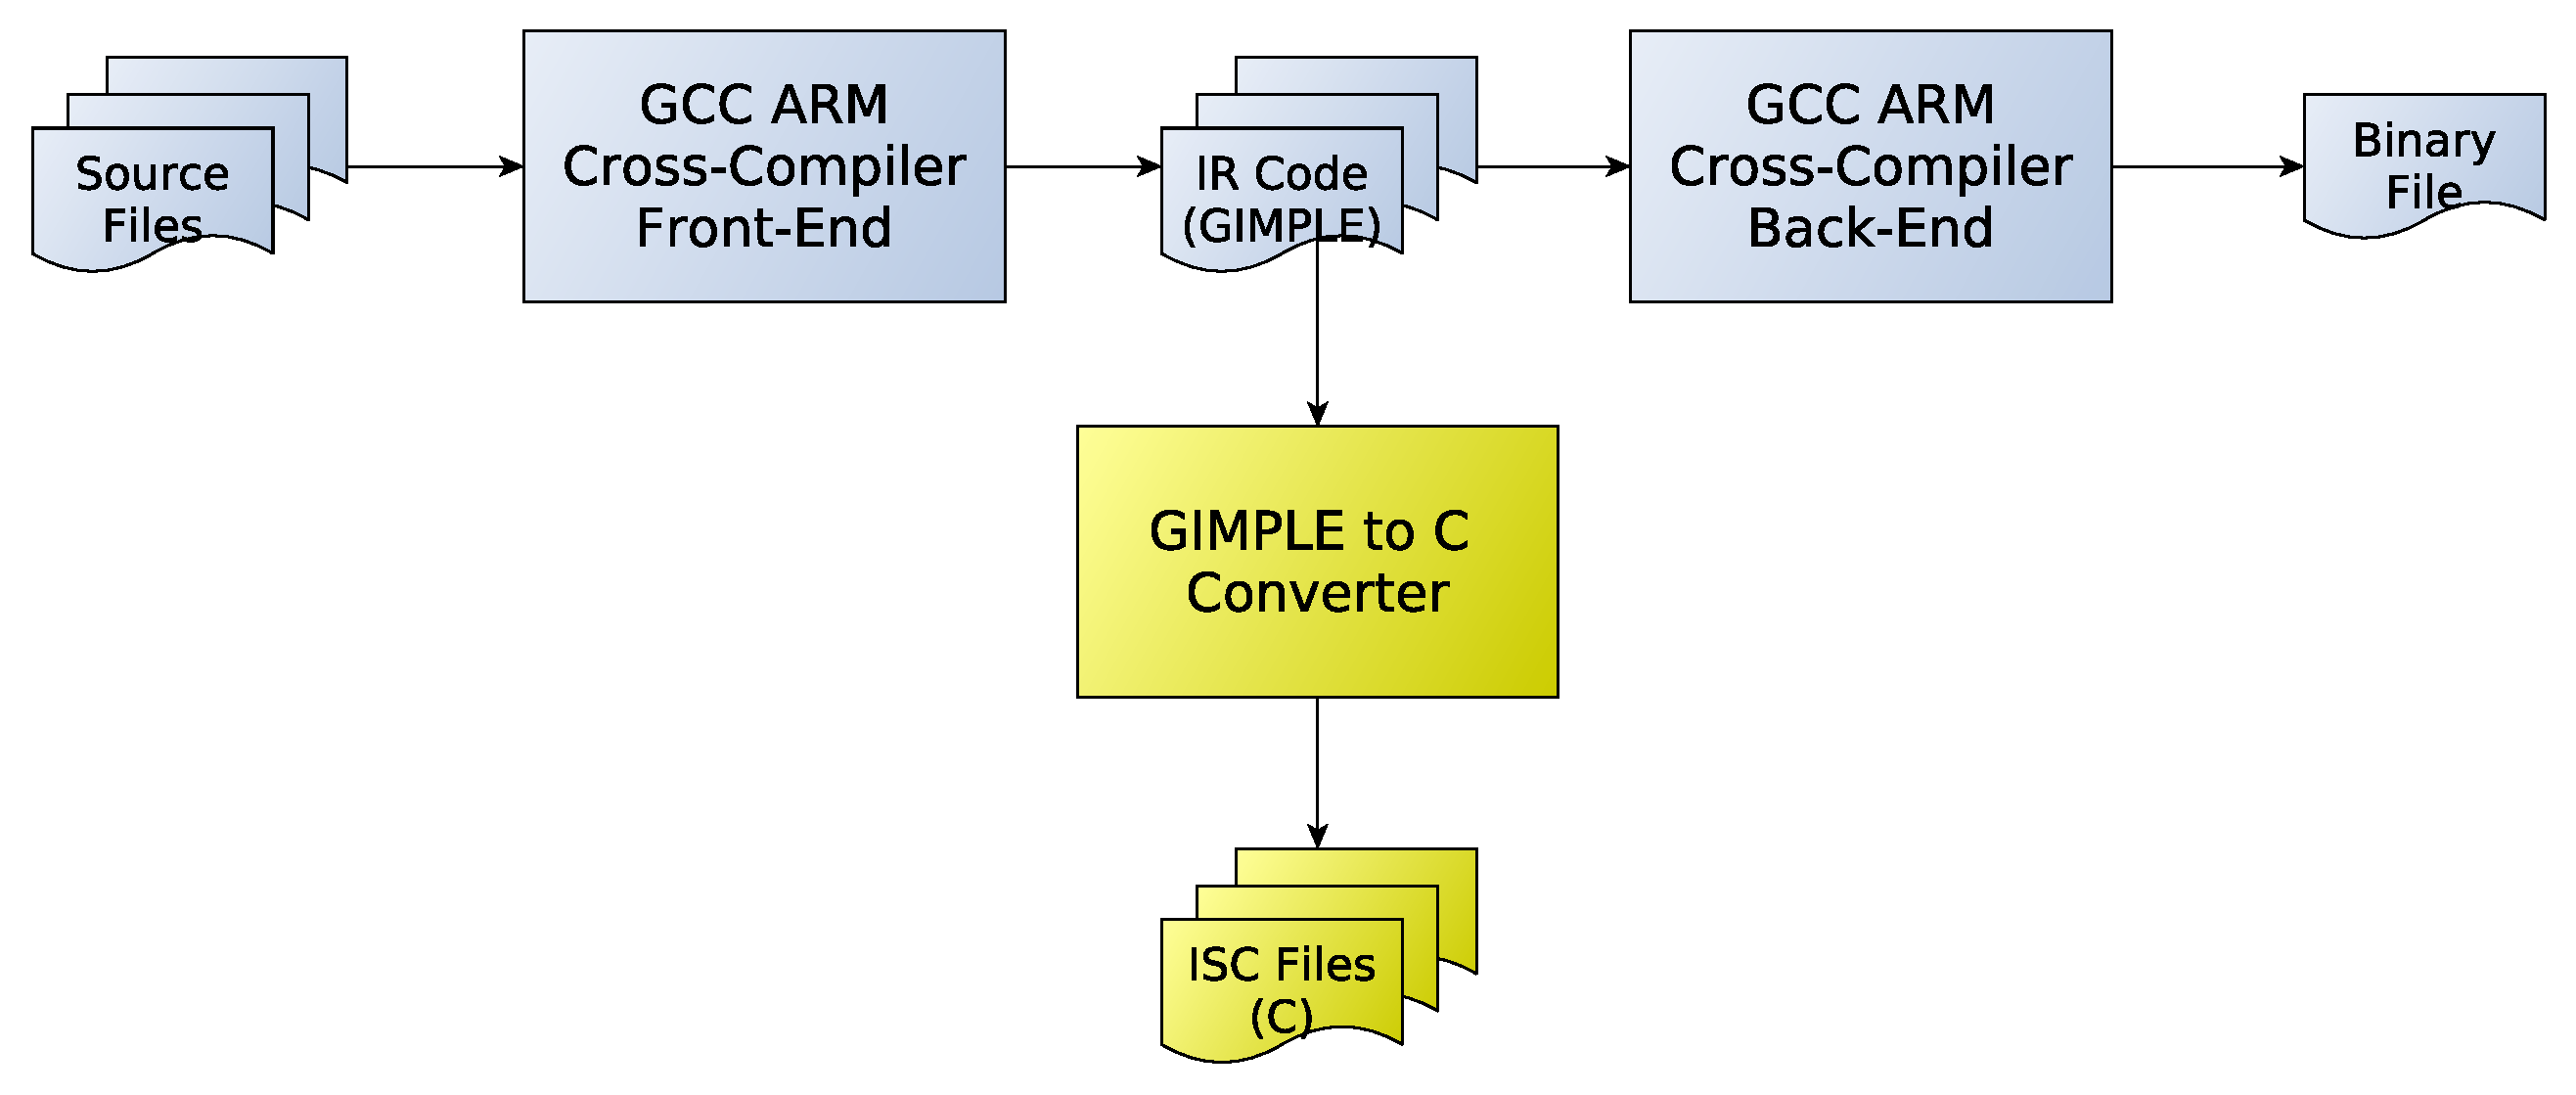
\includegraphics[width=.9\textwidth]{figures/ir2cConversion.pdf}
\caption{Conversion of Source Code to Intermediate Source Code}
\label{fig:ir2cConversion}
\end{figure}

Extracting mapping between \gls{isc} and binary code is comparatively easier. This is aided by the fact that \gls{isc} is easier to parse, as it uses simple \emph{if-else} constructs and \emph{goto} commands to implements loops. \gls{isc} is fairly easy to read and understand for the developer. Instrumentation is performed to the \gls{isc}. 

To aid understanding, the ISC will be referred to as the source code in further sections.

\section{Mapping between ISC and Binary Code}
Even between \gls{isc} and Binary Code, the control flow is significantly different. This is because processor dependent optimizations are not included in the ISC. Modern processors offer complex optimization features. These features are processor-dependent and can only be utilized by the compiler back-end.

Compiler optimizes code by moving instructions around. Sometimes new blocks will be created in the Binary Code. Using predication or conditional execution, the compiler may try to eliminate branching instructions. Blocks will be merged in doing so. A complete one to one mapping between basic blocks may often not exist. The mapping algorithm must take this into account, and find a mapping such that each basic block in the binary code maps to a basic block in the source code.

GDB provides mapping information, but was observed to be highly inaccurate. To perform accurate mapping, complex techniques have been proposed based on analysis of Data and Control Flow. In this project, the Control Flow Graphs (CFGs)\footnote{Control Flow Graph is a graph representing flow of control among basic blocks in the code. The nodes represent basic blocks, and the edges represent the possible flow of execution.} of \gls{isc} and binary code are analysed using a mapping algorithm. The approach is inspired from \cite{RBA2013}.

The mapping algorithm is based on the standard Graph Matching Algorithm using recursive Depth First Traversal. CFGs are extracted by parsing the source code and the binary code. To assist in mapping, a \textit{flow} value is calculated for each node in the graphs. The \textit{flow} value for a node is the sum of the \textit{flows} of the incoming edges to the node, which in turn is equally divided among the outgoing edges. The \textit{flow} value of the root node is 1. Only nodes with equal flow value can be mapped to each other.

The pseudo code of the \emph{mapping} function is presented in Algorithm \ref{algo:mapping}. The recursive function takes two nodes as parameter, and tries to find if the nodes map to each other. It checks that the nodes have the same \textit{flow} values, and returns \textit{False} if not. If the nodes have already been mapped to each other, the function returns \textit{True}. 

At this point, special handling for different compiler optimizations is done. Section [TODO] will illustrate the handling for Conditional Execution optimization that is frequently seen in the test set of benchmarks.

Hereafter, the successor sets of both nodes are created. To find successor nodes, only forward edges to are considered. Back edges representing loops are ignored. Two nodes can be mapped to each other, only if they have the same number of successor nodes. For each successor \emph{S\_src} in \emph{SS\_src}, a matching node in \emph{SS\_bin} is identified by recursively calling the \emph{mapping} function. 

The nodes map to each other, if a mapping can be found for all successor nodes. The algorithm tries to find matching path from the start node, to the exit node and creates mapping between the nodes on this path.

% http://tex.stackexchange.com/questions/163768/write-pseudo-code-in-latex
% TODO Complete algorithm
\begin{algorithm}[h!]
\caption{CFG Mapping Algorithm}\label{algo:mapping}
\begin{algorithmic}[1]
\Function{Mapping}{BB\_src, BB\_bin}
\If {\textit{flow}(BB\_src) != \textit{flow}(BB\_bin)}
\State \Return false
\EndIf
\\
\If {(BB\_src, BB\_bin) $\in$ MappingDict}
\State \Return true
\EndIf
\\
\State // Check for effects due to Compiler Optimization here
\\
\State SS\_src = \textit{Succ}(BB\_src)
\State SS\_bin = \textit{Succ}(BB\_bin)
\If {\textit{len}(SS\_src) != \textit{len}(SS\_bin)} 
\State \Return False
\EndIf
\\
\For {S\_src in SS\_src}
\For {S\_bin in SS\_bin}
\If {\textit{Mapping}(S\_src, S\_bin) == True}
\State break
\Else
\State continue
\EndIf
\EndFor
\State // Mapping could not be found for S\_src
\State \Return false
\EndFor
\\
\State // All children mapped; Input Nodes must map to each other
\State MappingDict $\leftarrow$ (BB\_src, BB\_bin)
\State \Return true
\\
\EndFunction
\end{algorithmic}
\end{algorithm}

The instrumentation tool generates graphical representation of the mapping between the CFGs. Mapping for some benchmarks, that were used to test the tool have been shown in [TODO].

\subsection{Handling of Conditional Execution Optimization}
\label{subsec:CondExec}
Conditional Execution or Branch Predication is a feature supported in some Instruction Set Architectures to mitigate the cost associated with conditional branching. Consider the following example to understand the performance impact of this feature.

Example \ref{ex:cIfElse} shows a simple \emph{if-then-else} construct written in C. The code checks if \emph{a} is greater than \emph{b}. If true, the value of \emph{a} is assigned to \emph{max}, else the value of \emph{b} is assigned to \emph{max}. Example \ref{ex:objIfElse} is representative of how the assembly code may look like without any optimization.

\begin{Example}[h]
\begin{lstlisting}
int max(int a, int b)
{
    int ret;
    if (a > b)
        max = a;
    else
        max = b;
    return ret;
}
\end{lstlisting}
\caption{Example C Code}
\label{ex:cIfElse}
\end{Example}

\begin{Example}[h]
\begin{lstlisting}
00008068 <max>:
    8068:       cmp     r1, r0
    806c:       ble     8078   
    8070:       mov     r0, r1
    8074:       b       807c
    8078:       mov     r0, r0
    807c:       bx      lr
\end{lstlisting}
\caption{Unoptimized Object Code}
\label{ex:objIfElse}
\end{Example}

Instructions take more than one cycle to execute. To improve throughput, execution unit in almost all processors is implemented as a multi-stage pipeline. Instructions are fed into the pipeline and executed in parallel.

The \emph{cmp} instruction on line 2 in Listing \ref{ex:objIfElse} is fetched by the first stage of the pipeline. While it is being decoded in the next stage of the pipeline, the branch instruction on line 3 has been fetched. Depending on the result of the compare instruction, the branch will be taken or not taken. The result of the compare instruction has not yet been evaluated. The processor cannot know with certainty which instruction to fetch after the branch instruction.

By assuming that the branch will not be taken, the processor fetches the \emph{mov} instruction on line 4. If the prediction is incorrect the pipeline must be flushed and \emph{mov} instruction on line 6 must be executed next. The pipeline flush leads to loss of multiple clock cycles.

This loss can be reduced by using Conditional Execution, when supported by the architecture. Each instruction can be predicated with a condition. The instruction is executed in the pipeline, but the result is only written back (or committed) if the condition evaluates to true. In the optimized code in Example \ref{ex:objOptimizedIfElse} the \emph{movge} instruction will be executed, but the value of \emph{r1} will be written to \emph{r0} only if the result of the compare instruction is "Greater than" or "Equal". A few clock cycles can be saved if the length of the conditionally executed block is small.

\begin{Example}[h]
\begin{lstlisting}
00008068 <max>:
    8068:       cmp     r1, r0
    806c:       movge   r0, r1
    8070:       movlt   r0, r0
    8074:       bx      lr
\end{lstlisting}
\caption{Optimized Object Code}
\label{ex:objOptimizedIfElse}
\end{Example}

The CFGs for the source code, and the unoptimized binary code have been represented in figures \ref{fig:cfgSrc} and \ref{fig:cfgUnopt}. The labels in the nodes represent line numbers for the corresponding basic blocks. These graphs are similar, and hence easy to map. 

However, in the optimized binary code the branching instructions are eliminated. The code is considered as a single basic block, as shown in the CFG in figure \ref{fig:cfgOpt}.

\begin{figure}[h!]
\centering
\begin{subfigure}[t]{.33\textwidth}
\captionsetup{margin=10pt}
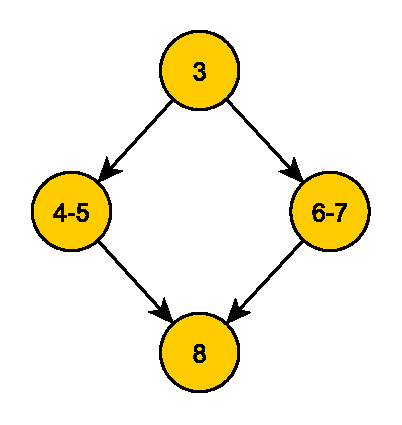
\includegraphics[width=\textwidth]{figures/CondExecSrcFlowChart.pdf}
\caption{Source Code}
\label{fig:cfgSrc}
\end{subfigure}%
~
\begin{subfigure}[t]{.33\textwidth}
\captionsetup{margin=10pt}
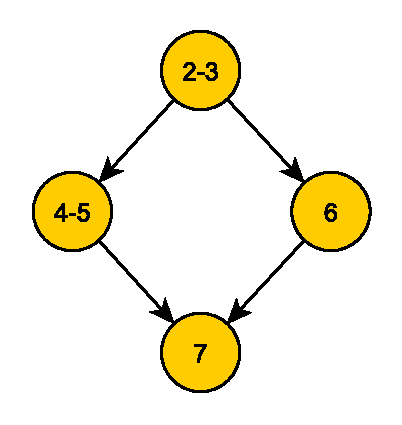
\includegraphics[width=\textwidth]{figures/CondExecObjUnoptFlowChart.pdf}
\caption{Unoptimized Binary Code}
\label{fig:cfgUnopt}
\end{subfigure}%
~
\begin{subfigure}[t]{.33\textwidth}
\centering
\captionsetup{margin=10pt}

\includegraphics[width=.5\textwidth]{figures/CondExecObjOptFlowChart.pdf}
\caption{Optimized Binary Code}
\label{fig:cfgOpt}
\end{subfigure}
\caption{Control Flow Graphs}
\end{figure}

To handle this optimization, the binary basic block is analysed to check if Conditional Execution Instructions have been used. The mapping algorithm maps all four blocks of the source code, to the single block in the binary code. 

\section{Annotation for Execution Cycles}
The annotation for number of cycles spent in execution of the instructions is done at a basic block granularity. A global variable \emph{execCycles} is declared. Cycles spent in executing each basic block in the binary code is estimated and annotated in the mapped basic block in source code. On entering the basic block, the annotated cycles for the block are added to \emph{execCycles}.

Most processors use a multi-stage pipelined execution unit. The cycles spent in executing instructions depends on the structure of the pipeline. Some instructions have data and control dependency on the previous instruction. For instance, an instruction may need as input the result generated by the previous instruction. This is known as interlocking and leads to pipeline stalls. To accurately estimate the number of cycles spent in executing the basic block the structure of the pipeline and effects of interlocking must be taken into consideration.

Instructions from the binary are parsed sequentially and simulated on the pipeline in a cycle accurate fashion. For each basic block, it is assumed that the pipeline is initially empty, which may not be the case and will be accounted for later. It is also assumed that all the data needed by the instructions is available with no latency. The cycles spent in fetching the data from memory will also be accounted later. Interlocking between instructions is identified and appropriately accounted. 

The total number of cycles as calculated from the simulation is annotated to the corresponding basic block in the source code, as illustrated in the example below. On entering the basic block, global variable \emph{execCycles} is incremented by the number of cycles spent in executing the basic block. This is done each time the basic block gets executed.

%TODO : Add Exapmle

\subsection{Branch Prediction}
To calculate the cycles spent in execution, it was assumed that the pipeline is empty at the start of each basic block. This may not always be the case. This will be taken into account here.

Conditional branching is implemented in binary code as a compare instruction followed by a conditional branch instruction. The branch is taken depending on the result of the compare instruction. In a pipelined execution unit, instructions are executed in parallel. The result of the compare instruction may not be available in time, to decide the instruction to be fetched after the branch instruction. The processor uses \gls{bpu} to predict the outcome of the branch instruction. The appropriate instructions are loaded into the pipeline.

If the prediction is incorrect, the pipeline must be flushed and the correct instruction to be executed next must be fetched. If the prediction is correct, a few cycles are saved. To account for the saved cycles, the \gls{bpu} is simulated.

The \gls{bpu}, uses heuristics to predict the outcome of a branch instruction. A state machine is implemented to predict the outcome of the branch. A table maintains the history of branch instructions seen in the recent past. The address of the branch instruction is stored along with a 2-bit state information. The states and transitions for each branch are shown in the state machine diagram in figure 
\ref{fig:bpuSMD}.

\begin{figure}[h]
\centering
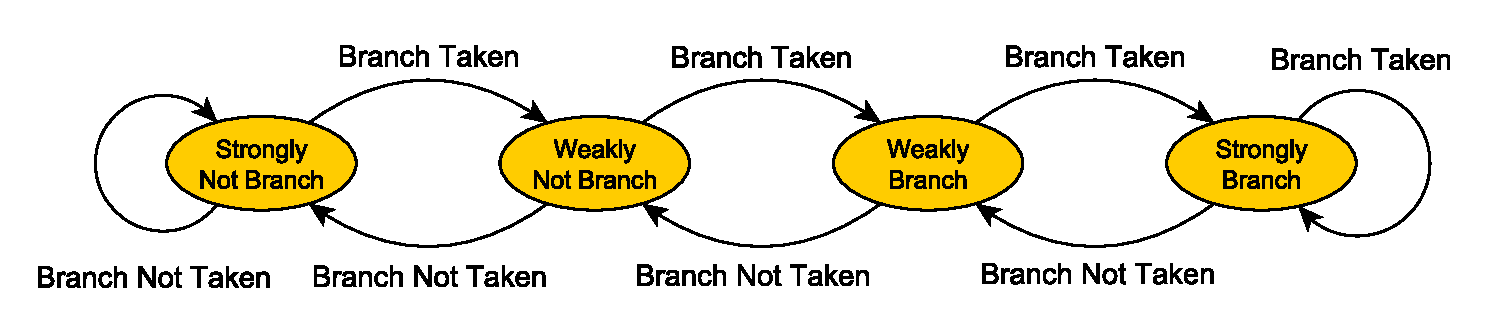
\includegraphics[width=.8\textwidth]{figures/BranchPredictionSMD.pdf}
\caption{State Machine Diagram implemented in the Branch Prediction Unit}
\label{fig:bpuSMD}
\end{figure}

The \gls{bpu} predicts that the branch will not be taken, when the current state is either "Strongly Not Branch" or "Weakly Not Branch". In the other states, the \gls{bpu} predicts that the branch will be taken.

When a branch instruction is loaded into the pipeline, the \gls{bpu} checks if the information for the branch is present in the history table. If an entry is not found, the processors predicts that the branch will not be taken. An entry is added to the table with state "Strongly Not Branch". When the branch is found in the history table, the prediction is made based upon the current state of the entry. The state of the entry is changed accordingly, when the outcome of the branch is known.

A Branch Prediction Simulator has been developed which uses the same algorithm. It offers the API as shown in Listing [TODO]. For each basic block in the binary code, the mapped basic block in source code is instrumented to call this API, as illustrated in example in listing [TODO]. 

The start and end address of the basic block is parsed as a parameter. This information is extracted from the binary code. When the function is called, the simulator checks whether the branch from the previous block to current block would have been predicted by the \gls{bpu}. It returns \emph{True} if the branch would have been predicted correctly, in which case a few cycles would be subtracted from \emph{execCycles}. 

\section{Annotation for Memory Access}
The cycles spent in fetching data and instructions from the memory must be accurately estimated. To do this, a Cache Simulator has been implemented. 

\subsection{Cache Simulator}
Most processors use a hierarchy of low-latency cache memories to improve performance by reducing the time spent in fetching data from memory. Caching has a significant impact on performance. To take this into account, an accurate simulation of the cache hierarchy needs to be done.

The Cache Simulator emulates the caching hierarchy of the target processor. It keeps a track of the data stored in the caches. Whenever a memory access is performed, the simulator checks whether the data can be fetched from the caches. If the data is not found in any cache, it must be fetched from the memory. The simulator returns the number of cycles that would be spent in performing the memory access on the target processor.

Most processors use separate cache for Data and Instructions. The cache simulator offers the API mentioned in snippet \ref{snip:csimAPI} to simulate different types of memory accesses.

\vspace*{10pt}
\begin{Snippet}[h]
\begin{lstlisting}[numbers=none]
/**
 * @brief Function to simulate Data Cache Access.
 *
 * @param Address of the data to be fetched
 * @param True, if read access
 *         False, if write access
 * @param Detailed result for trace
 *
 * @return Number of cycles spent in performing access.
 */
unsigned long long simDCache(unsigned long address,
                                unsigned int is_read_access,
                                struct csim_result_t *csim_result);
                                
/**
 * @brief Function to simulate Instruction Cache Access.
 *
 * @param Start Address of the basic block
 * @param Size of the basic block in Bytes
 * @param Detailed result for trace 
 *
 * @return Number of cycles spent in performing access.
 */
unsigned long long simICache(unsigned long address,
                                unsigned long size,
                                struct csim_result_t *csim_result);
\end{lstlisting}
\caption{API provided by Cache Simulator}
\label{snip:csimAPI}
\end{Snippet}

For each data access in the application, annotation is done in the source code to call function \emph{simDCache} and trigger Data Cache simulation. The address of the data being fetched is provided as parameter, along with a flag to signify whether it is a read or write access. Simulation of Instruction Cache is done at basic block granularity. \emph{simICache} is called, with the start address of the basic block and the size of the basic block in bytes as parameters. Number of cycles spent in performing the memory access is returned by the cache simulator.

The third parameter to both \emph{simDCache} and \emph{simICache} is an address to an object of type \emph{struct csim\_result\_t} where detailed result of the simulation is stored. This data will be useful for estimating power consumption, as will be discussed later.

Caches may have varying parameters and features such as,
\begin{itemize} \itemsep -6pt
\item Sizes
\item Approach for Associativity of Data (Direct Mapped, N-way Set Associative)
\item Hierarchy (multiple levels of caching)
\item Replacement Policies
\end{itemize}

The cache simulator has been designed in a modular fashion. Platform specific implementation of the cache may be plugged into the API. Architects can alter specific parameters of the cache and analyse the impact on performance, without having to instrument the code again.

\section{Instruction Cache Simulation}
For estimating cycles spent in fetching the instructions from memory, instrumentation for instruction cache simulation is performed at the basic block granularity. 

For each basic block in the cross-compiled binary code, the address of the first instruction in the block and size of the block in bytes is extracted. Note that since the binary is compiled to be run on Bare-Metal, the load address of the binary was decided at compile time. The addresses of instructions extracted from the binary, were physical addresses where the instructions will reside in the memory of the target system.

The corresponding basic block in the source code is identified from the mapping information. Instrumentation is performed at the beginning of the basic block, and the instruction access is simulated using the API provided by the cache simulator.

As illustrated in listing [TODO], the return value from \emph{simICache} is accumulated to the global variable \emph{memAccessCycles}.

\section{Data Cache Simulation}
The example shown in Section [TODO] was simplified for illustration. It had a flaw which will result in inaccuracy of estimation. To simulate load operation to fetch elements of \emph{array}, the address of \emph{array} at run-time from the Host Machine was used. For accurate estimation, data access must be simulated using target addresses. This is important since the host and target memory systems may vary significantly. For instance, the host and target system may use different sizes for basic data types, like integers. This will lead to severe inaccuracy when accessing a sequence of elements from an array of integers. 

Resolving the address of load/store operation cannot be done by static analysis of the code. The process to do this is inspired from research published in [TODO] and is called Memory Access Reconstruction. 

\subsection{Memory Access Reconstruction}
Memory Access Reconstruction is the technique to resolve address of each load/store instruction as it would occur on the target processor. The address is then used for accurately simulating data cache access. 

The steps needed for Memory Access Reconstruction are as follows

\begin{itemize} \itemsep -6pt
\item Resolve address of each variable used in the program.
\item Analyse the binary code to identify the variable being accessed by each load/store instruction.
\item Parse the source code to extract information for accurate instrumentation of Data Access
\end{itemize}

\subsubsection{Resolve address of each variable}
An application may use different types of variables. The technique to resolve address of each variable is described below. 

\paragraph{Global Variables}
Global Variables are accessible by all functions, and are stored in the Data Section of the application memory. The physical addresses of the global variables are decided at compile time. The address, size and type of each Global Variable is extracted by static analysis of the binary using GDB. 

For each global variable \emph{var}, another global variable \emph{var\_addr} is declared by instrumentation. The address of the global variable on the target system is stored in this variable. This address is later used for simulating access to the global variable. Refer to the example \ref{ex:GlobVarInst}.

\vspace*{15pt}
\begin{Example}
\begin{lstlisting}
int globalVar[20];
`unsigned long globalVar_addr = 0x7c8;` // Address of global variable

void foo ()
{
    ...
}
\end{lstlisting}
\caption{Instrumentation to resolve address of Global Variables on Target Device}
\label{ex:GlobVarInst}
\end{Example}

\paragraph{Local Variables}
Local Variables are defined inside a function definition, and are only accessible inside the function. Memory for Local Variables is only allocated when the function is called, and is located in the stack frame of the function. The actual physical address of the local variables can not be resolved by static analysis, as the stack grows and compacts at run-time. However, the address of each local variable relative to the value of the stack pointer, can be known.

If the value of the stack pointer is known, the relative address can be added to it to resolve the physical address of the local variable. Whenever a function is called, the stack frame of the function is pushed to the stack. The stack frame is popped when the function returns. To keep track of the stack pointer at run-time, a global variable \emph{CSIM\_SP} is declared and initialized with the initial value of the stack pointer. The stack frame size of each function is extracted by static analysis of the binary. \emph{CSIM\_SP} is incremented at the beginning of each function by the stack frame size of the function and decremented before the function returns.

Example \ref{ex:LocalVarInst} illustrates the annotations needed to resolve the physical address of local variables.

\begin{Example}
\begin{lstlisting}[label=lst:LocalVarInst]
`unsigned long CSIM_SP = 0x1ff280;` // Intial Value of Stack Pointer

void foo ()
{
    double localVar;
    `unsigned long localVar_addr = 0x08;` // Address relative to SP

    `CSIM_SP = CSIM_SP + 0x16;` // Increment by size of stack frame
    
    ...
    
    `CSIM_SP = CSIM_SP - 0x16;` // Decrement by size of stack frame
    
    return;
}
\end{lstlisting}
\caption{Instrumentation to resolve address of Local Variables on Target Device}
\label{ex:LocalVarInst}
\end{Example}

\paragraph{Dynamically Allocated Memory}
Dynamically Allocated Memory is stored in the Heap Section. To allocate and free heap memory, the application uses API provided by system libraries. The memory allocation algorithm of the target system needs to be emulated at run-time of simulation, to resolve physical addresses of dynamically allocated memory. This approach is discussed in [TODO]. However, this is complicated to achieve, and has been ignored for this project. Only benchmark applications that do not use Dynamically Allocated Memory can be used. The project can later be extended to include this functionality.

\subsubsection{Analyse binary code for identifying load/store operations on variables}
To identify which variable is being accessed, the binary code is partially simulated. A simple simulator is developed in Python, which maintains the state of each register in the target processor. Starting from the main function, each instruction in the binary code is parsed and state of the registers is updated. In this simulation, the branching instructions are ignored. This means, each instruction will only be parsed once. 

When function calls are identified, the current state of the registers is stored. This state will be used when simulating the called function. This is done to keep track of function parameters that are passed as values in registers. For parameters being passed in the stack, this approach does not correctly work. A queue is maintained for each function that is called. Each function is simulated with the initial state of registers that was recorded when the function was first called. Note that each function will only be simulated once, and subsequent calls to the function were ignored.

The illustration in figure \ref{fig:partialSimulator} shows how this works. The code from the simple example in section \ref{sec:SimpleExample} has been used for illustration. The binary code of the \emph{sum} function is shown on the left. On the right, the symbol table shows the address of the global variable, \emph{globVar}. 

The state of the registers is shown when the function was called. Address of the \emph{globVar} was sent as a parameter to the function in register \emph{r0}. The values in the rest of the registers are arbitrary. The state of the registers is updated after parsing each instruction in the code. On line 4, a load instruction is seen. The address in \emph{r0} is indexed by the value in \emph{r3}, and the data is read into \emph{r1}. The address belongs to global variable \emph{globVar}. 

\begin{figure}[h]
\centering
\includegraphics[width=\textwidth]{figures/ParitalSimulator.png}
\caption{Illustration of the Partial Functional Simulator used to extract address of each load/store instruction in the binary code}
\label{fig:partialSimulator}
\end{figure}

By doing this simulation, the address of each load/store instruction can be extracted. This information helps in identifying which variable is being accessed by the load/store instruction. 

\begin{itemize}
\item If the address belongs to Data Section, the instruction must be accessing a Global or Static Variable. Addresses of Global and Static Variables were extracted in the previous stage. The variable being accessed can be identified. 
\item If the address belongs to the Stack Space, it could be accessing a local variable. The variable being accessed is again identified from the information collected in the previous phase. Additionally, the stack space is used to spill registers. The load/store instruction could be associated with this operation. This can be distinctively identified, if no local variable is located on this address.
\end{itemize}

The memory accesses performed in each basic block in the binary code are recorded. Instrumentation for simulating these accesses will be done in the corresponding basic blocks in the source code. 

This approach has certain limitations. It may fail, in the presence of some pointer dereferencing operations. When the variable being accessed by a load/store instruction is not identified, appropriate hints are provided in the log to enable the user of the tool to manually instrument the code.

Note, that in this step only the variables being accessed were identified. In the example shown above \emph{globVar} is an array of integers. Elements of this array are accessed sequentially in the code, but this can not be identified in this step. To correctly instrument the Data Cache Access, the index being added to the base address of an array must be known. This information can only be extracted by parsing the source code.

\subsubsection{Parse Source Code}
By analysing the binary code, variables accessed in each basic block were identified. Additionally, load/store instructions associated with register spilling were distinctly identified. Instrumentation for register spilling is straight forward.

In this stage, the focus is to identify the statement in source code which causes memory access to a variable. By parsing this statement, the exact address being accessed can be identified. A custom C Parser is implemented in Python to parse the Instrumented Source Code (ISC). Conversion of source code to ISC helps here, because ISC is easier to parse. The parser returns a list of variables being accessed by the statement, along with other information like index expression and whether it is a read or write operation.

Instrumentation for matching memory accesses found in source code and binary code is done. Instrumentation for local and global variables is handled in different ways as is shown below.

Another typical case must be taken into consideration. In the simple example in Section \ref{sec:SimpleExample}, pointer to an array is passed as a parameter to the function. By simulating the binary code, access to Global Variable \emph{globVar} was identified. However, the function \emph{sum} may be called with a pointer to any other array. Special handling needs to be done for such cases, when pointers are sent as function parameters.

The approach used in this project, is to modify the signature of each function that takes pointers as arguments. For each pointer argument \emph{ptr}, a new argument is added \emph{ptr\_addr}. The calling function is accordingly modified, to provide address of the variable on the target processor. When \emph{ptr} is dereferenced, data cache access is simulated using \emph{ptr\_addr}. Refer to the following example for this annotation.






